%---------
% place your email id between the braces so that your homework has a name
\def\yourname{}
% -----------------------------------------------------
\def\duedate{4/5/24}
\def\duelocation{via \href{https://www.gradescope.com/courses/753885}{Gradescope}}
\def\hnumber{3}
\def\prof{Lorenzo Orecchia}
\def\course{\href{https://canvas.uchicago.edu/courses/56880}{CMSC 27200 - Spring 2024}}
%-------------------------------------

\documentclass[10pt]{article}
\usepackage[colorlinks,urlcolor=blue]{hyperref}
\usepackage[osf]{mathpazo}
\usepackage{amsmath,amsfonts,graphicx}
\usepackage{latexsym}
\usepackage{subfig}
\usepackage{algpseudocode}
\usepackage[shortlabels]{enumitem}
\usepackage{algorithm}
\usepackage{listings}
%\usepackage[top=1in,bottom=1.4in,left=1.5in,right=1.5in,centering]{geometry}
\usepackage{fullpage}
\usepackage{color}
\definecolor{mdb}{rgb}{0.3,0.02,0.02} 
\definecolor{cit}{rgb}{0.05,0.2,0.45}
\usepackage{wrapfig}
%\pagestyle{myheadings}
\markboth{\yourname}{\yourname}

\thispagestyle{empty}

\newenvironment{proof}{\par\noindent{\it Proof.}\hspace*{1em}}{$\Box$\bigskip}
\newcommand{\qed}{$\Box$}
\newcommand{\alg}[1]{\mathsf{#1}}
\newcommand{\handout}{
   \renewcommand{\thepage}{H\hnumber-\arabic{page}}
   \noindent
   \begin{center}
      \vbox{
    \hbox to \columnwidth {\sc{\course} --- \prof \hfill}
    \vspace{-2mm}
    \hbox to \columnwidth {\sc due \MakeLowercase{\duedate} \duelocation\hfill {\Huge\color{mdb}H\hnumber.\yourname}}%
      }
   \end{center}
   \vspace*{2mm}
}
\newcommand{\solution}[1]{
\vspace{2mm}

\noindent Collaborators:

\vspace{5mm}

\medskip\noindent{\color{cit}\textbf{Solution:} #1}}

\newcommand{\bit}[1]{\{0,1\}^{ #1 }}
\newcommand{\extraspace}{\medskip\noindent{\color{cit} Extra space for your solution}\newpage}
%\dontprintsemicolon
%\linesnumbered=
\newtheorem{problem}{\sc\color{cit}Problem}
\newtheorem{lemma}{Lemma}
\newtheorem{theorem}{Theorem}
\newtheorem{definition}{Definition}
\newtheorem{claim}{Claim}


\begin{document}
\handout
\begin{itemize}
\item The assignment is due at Gradescope on \duedate.

\item A LaTeX template will be provided for each homework. You are strongly encouraged to type your homework into this template using \LaTeX.  If you are writing by hand, please fill in the solutions in this template, inserting additional sheets as necessary. This will help facilitate the grading.

\item You are permitted to discuss the problems with up to 2 other students in the class (per problem); however, {\em you must write up your own solutions, in your own words}. Do not submit anything you cannot explain. If you do collaborate with any of the other students on any problem, please list all your collaborators in the appropriate spaces.

\item Similarly, please list any other source you have used for each problem, including other textbooks or websites.

\item {\em Show your work.} Answers without justification will be given little credit.

\item Your homework is \textit{resubmittable}. Please refer to the course syllabus on Canvas for a more detailed description of this. For any problem that you have not changed from your last submission, please make sure to indicate this in your submission to help our graders grade faster. 

\end{itemize}


%%%%%%%%%%%%%%%%%%%%%%%%%%%%%%%%%%%%%%%%%%%

%%%%%%%%%%%%%%%%%%%%%%%%%%%%%%%%%%%%%%%%%%%

\newpage
\begin{problem}[Recursive functions]

For the following recursive functions, compute their $O(\cdot)$ complexity:
\begin{enumerate}
    \item $T(n) = 7 T(n/2) + 4n$
    \item $T(n) = 16 T(n/4) + n^2$
    \item $T(n) = 2 T(n/4) + \sqrt{n}$
    \item $T(n) = T(n - 1) + n^2$
\end{enumerate}
\end{problem}
\solution{ 
    We can compuite complexity by Master Theorem as we have the functions in the form of $aT(\frac{n}{b}) + O(n^d)$.
    \begin{enumerate}
        \item $T(n) = 7 T(n/2) + 4n$: We have $a = 7$, $b = 2$ and $d = 1$. As $7 > 2^1$, we have $T(n) = O(n^{\log_2 7})$.
        \item $T(n) = 16 T(n/4) + n^2$: We have $a = 16$, $b = 4$ and $d = 2$. As $16 = 4^2$, we have $T(n) = O(n^2 \log n)$.
        \item $T(n) = 2 T(n/4) + \sqrt{n}$: We have $a = 2$, $b = 4$ and $d = 0.5$. As $2 = \sqrt{4}$, we have $T(n) = O(\sqrt{n}\log n)$.
        \item $T(n) = T(n - 1) + n^2$: Master Theorem is not applicable, but this recursive function can be transformed to $T(n) = T(n-1)+n^2 = (T(n-2)+ T(n-1)^2) + n^2 = \dots = T(1) + 2^2 + \dots +n^2$
            which can be computed as $\frac{n(n-1)(2n+1)}{6}$, which has $O(n^3)$.
    \end{enumerate}
}

\newpage
\extraspace
\newpage

\iffalse
\begin{problem}[The Billy Problem]
This problem is due to Professor Drucker who was inspired by The Family Circus.\\  
\\
Billy, a 7-year-old kid, is let loose in a park, which is an $N$-by-$N$ grid of cells $(x, y) \in [N]\times [N]$. His starting location is the Southwest corner $(x, y) = (1, 1)$. He takes a walk in the park, always moving from a square to an adjacent square in one of the four cardinal directions.  He never leaves the park, and never visits the same square twice.  Eventually he ends up napping somewhere in the park. \\

We are given the $N$-by-$N$ matrix $A$, whose entries are 
\begin{enumerate}
\item $A[i, j] = *$ if Billy never visits cell $(i, j)$.
\item $A[i, j] = \uparrow$ if Billy visited cell $(i, j)$ and departed upwards.
\item $A[i, j] = \leftarrow$ if Billy visited cell $(i, j)$ and departed in the leftwards direction.
\item $A[i, j] = \downarrow$ if Billy visited cell $(i, j)$ and departed downwards.
\item $A[i, j] = \rightarrow$ if Billy visited cell $(i, j)$ and departed in the rightwards direction.
\item $A[i, j] = BILLY$ if Billy is napping in cell $(i, j)$.
\end{enumerate}

For example, $A[1, 1]$ will contain an arrow indicating the first step Billy took after entering the park (unless he stopped to nap immediately).

Give an algorithm (either with pseudocode or in words) that makes only $O(N)$ queries to the matrix $A$, and locates Billy. In other words, your algorithm should only read $O(N)$ entries of the matrix. You should give a sketch that your algorithm works and only makes $O(N)$ queries, but you do not need to give a rigorous proof. You can get an $S$ for an algorithm which uses $O(N \log N)$ queries.

\end{problem}

\solution{
Your solution here.
}
\section{Tracking Drones (15 points)}

With drones becoming more prominent, it is useful to be able to quickly find their position. However your drone is no longer transmitting GPS data, but it connects to cellular towers as it moves. You cannot ask the cellular tower network where your drone is, but each cellular tower will answer you if your drone is still connected to it \textbf{or} tell you to which tower and at what time it was handed over. 

The cellular towers are arranged in an $N$-by-$N$ grid of cells $(x, y) \in [N]\times [N]$. The drone's initial position is in the southwest corner $(x, y) = (1, 1)$ of the grid. The drone will stay in the grid, always moving from a square to an adjacent square in one of the four cardinal directions. It never leaves the grid, and never visits the same cell twice.

You are given a direction matrix $A$ and a time matrix $T$, both of size $N$-by-$N$. The entries in $A$ are as follows:
\begin{itemize}
\item $A[i, j] = \ *$ if the drone never visits cell $(i, j)$.
\item $A[i, j] = \ \uparrow$ if the drone visited cell $(i, j)$ and departed upward. 
\item $A[i, j] = \  \leftarrow$ if the drone visited cell $(i, j)$ and departed in the leftward direction.  
\item $A[i, j] = \ \downarrow$ if the drone visited cell $(i, j)$ and departed downward. 
\item $A[i, j] = \ \rightarrow$ if the drone visited cell $(i, j)$ and departed in the rightward direction.  
\item $A[i, j] = \ \texttt{DRONE} $ if the drone is connected to the tower in cell $(i, j)$.
\end{itemize}

The entries in $T$ are as follows:

\begin{itemize}
    \item $T[i,j] = \ -1$ if the drone has never left cell $(i,j)$
    \item $T[i,j] = t_{i,j}$ otherwise, where $t_{i,j}$ is the time that the drone left cell $(i,j)$
\end{itemize}

For example, if the drone leaves the southwest corner of the grid, $A[1, 1]$ will contain an arrow indicating which cellular tower the drone was handed over to. $T[1,1]$ will contain the timestamp of when the drone was handed to the new cellular tower. 

You may assume times are represented by integers and are comparable using standard operators (e.g., $\leq$, $\geq$, etc). 


\begin{enumerate}[(a)]
    \item (6 points) Write \textbf{pseudocode} for an algorithm that makes only $O(N)$ queries to the matrices $A$ and $T$ and locates the drone. In other words, your algorithm should only read $O(N)$ entries of the matrix. (A maximum of 2 points will be given for correct $O(N \log N)$ algorithms.)
    \item (6 points) Prove the correctness of your algorithm. State your base case and state the invariant that your algorithm maintains. 
    \item (3 points) Argue that your algorithm makes $O(N)$ queries.
    % \item (6 points) Give a sketch that your algorithm works and only makes $O(N)$ queries, but you do not need to give a rigorous proof.
    % \item (1 point) Now assume that the clocks in the cellular towers are all inaccurate. Without using the time information, describe briefly how you can still find the position of the drone in $O(N)$ queries.
\end{enumerate} 

(\textit{Credit}: This problem is due to Professor Andrew Drucker who was inspired by The Family Circus.)

\newpage
\extraspace
\fi

%%%%%%%%%%%%%%%%%%%%%%%%%%%%%%%%%%%%%%%%%%%

%%%%%%%%%%%%%%%%%%%%%%%%%%%%%%%%%%%%%%%%%%%

\newpage
\begin{problem}[Mafia Game]
A group of $n > 2$ friends are playing a game of Mafia. In each round of this game, the $n$ players can select any subset of the $n$ players to interrogate. Some number of the players are \textbf{Mafia}, and they will be revealed during the interrogation.

Denote by $P = \{P_1, P_2, \ldots P_n\}$ the set of $n$ players in the game. We may represent the interrogation as a function $I$ that takes as input any non-empty subset of $P$ and outputs a boolean in $\{\textsc{True}, \textsc{False}\}$ indicating whether the subset contains a Mafia member. More formally, if $P_i$ is Mafia, then $P_i \in P' \implies I(P') = \textsc{True}$.  
\begin{enumerate}[(a)]
    \item Suppose that there is only one Mafia member among the $n$. Provide a description (in words) of a divide-and-conquer procedure that allows the players to identify the mafia member in $O(\log n)$ interrogations. 
    \item Provide a proof sketch that this procedure always finds the Mafia. 
    \item Provide a proof sketch that your procedure from part (a) only takes $O(\log n)$ tests.
    \item Provide a formal proof that no procedure can guarantee finding the Mafia member in less than $\lfloor \log_2 n \rfloor$ interrogations. 
    \item (Bonus - Just to think about, no need to submit anything.) Suppose the Mafia member knows your procedure for picking subsets, and can successfully lie in $k$ interrogations (for some constant $k$). Obviously, if we just run each interrogation from (a) $k+1$ times, we'll find the Mafia. That seems redundant though. Is there a way for us to guarantee that we'll identify the Mafia in less than $(k+1)\log n$ interrogations? 
\end{enumerate}
Suppose instead that there are two Mafia in the group of $n$ players. Furthermore, they can cover each other's tracks in the interrogation: if both are in the same interrogation, then the players won't be able to detect that they are Mafia!

Formally, there exist two players $P_i$ and $P_j$ with $i \neq j$ such that
    \[
    I(P') = 
    \begin{cases}
        \textsc{False} & \text{If neither $P_i$ nor $P_j$ are in $P'$}, \\
        \textsc{True} & \text{If exactly one of $P_i$ or $P_j$ are in $P'$}, \\
        \textsc{False} & \text{If both $P_i$ and $P_j$ are in $P'$}. \\
    \end{cases}
    \]
\begin{enumerate}
    \item[(f)] Describe a procedure for selecting subsets to interrogate that allows the players to identify both Mafia in $O(\log n)$ interrogations. You may invoke your algorithm from part (a).
 
    \item[(g)] Sketch a proof that your procedure for part (d) is correct.
    \item[(h)] Sketch a proof that your procedure from part (d) takes $O(\log n)$ interrogations.
\end{enumerate}
\end{problem}

\solution{ 
    \begin{enumerate}[(a)]
        \item Split the $n$ players into two roughly equal groups, each of size $\frac{n}{2}$. Interrogate both groups. If group A contain a Mafia member, then the Mafia member 
            is in group A. Otherwise, the Mafia member is in group B. Without losing generality, we can assume that the Mafia member is in group A. Repeat the process with group A 
            to divide two groups and interrogate them. Continue this process until we have only one player left, which is the Mafia member. This process takes $O(\log n)$ interrogations as each step halves the group size.
        \item At each step, we are able to halve the group size, and one of these subgroups is eliminated based on the interrogation result. This process is repeated until we have only one player left, which is the Mafia member. 
            As we assume there is only one Mafia member, and since the Mafia member cannot be eliminated in any interrogation, we can guarantee that our procedure eventually isolate the Mafia member.
        \item Each interrogation will halve the group size. Starting with $n$ players, after the first interrogation we have $n/2$ players, after the second interrogation we have $n/4$ players, and so on. After $k$ interrogations, we have $n/2^k$ players. The worst case to find the Mafia number is the $n/2^k$th player is the Mafia,
            so we have $n/2^k = 1$. This gives us $k = \log_2 n$, and therefore $O(\log n)$.
        \item We can prove this by contradiction. Suppose there is a procedure that can find the Mafia member in less than $\lfloor \log_2 n \rfloor$ interrogations.
            This means that the procedure can find the Mafia member in $k$ interrogations, where $k < \lfloor \log_2 n \rfloor$ as we don't want players to remain after $k$ interrogations. Therefore, the procedure can find the Mafia member in $2^k < n$ players. 
            However, since there is only one Mafia member, and the Mafia member can be in any of the $n$ players, we cannot guarantee to find the Mafia member in less than $\lfloor \log_2 n \rfloor$ interrogations.
        \item (Thoughts) Introduce more reduncancy and see the pattern?
        \item Assign each player a unique number from $0$ to $n-1$ in binary representation. For each bit, we divide the players into two groups based on the bit value. For each bit position, if the interrogation returns True, we record the bit position and move on to the next bit position until Mafia members can be distinctly identified.
        \item Since each player has a unique binary identifier, there is guaranteed to be at least one bit position that differentiates any two players, including the two Mafia members. By iterating through all bit positions and dividing players based on these, you eventually find bit positions where the Mafia members are separated into different groups
        \item As we need to iterate through all bit positions, the number of bits needed to identify all players is $\log_2{n}$. For each bit position, we divide the players into two groups and interrogate both. Therefore we need $2\log_2{n}$ interrogations, which gives us $O(\log n)$.
    \end{enumerate}
}

\newpage
\extraspace

%%%%%%%%%%%%%%%%%%%%%%%%%%%%%%%%%%%%%%%%%%%

%%%%%%%%%%%%%%%%%%%%%%%%%%%%%%%%%%%%%%%%%%%

\newpage
\begin{problem}[Tilings] 
Consider a square $N \times N$ grid where $N = 2^k$ is a power of $2$, and imagine placing $L$-shaped domino pieces of area 3 on this grid. A \textbf{tiling} of the grid is a way of placing the pieces so that no two pieces overlap and every single grid cell is covered. In this problem you will be tasked with describing a procedure (an algorithm!) to cover the grid using only these $L$-shaped pieces. In the input grid, one square is excluded, and doesn't need to be covered by any domino piece.
\begin{figure}[H]
    \centering
    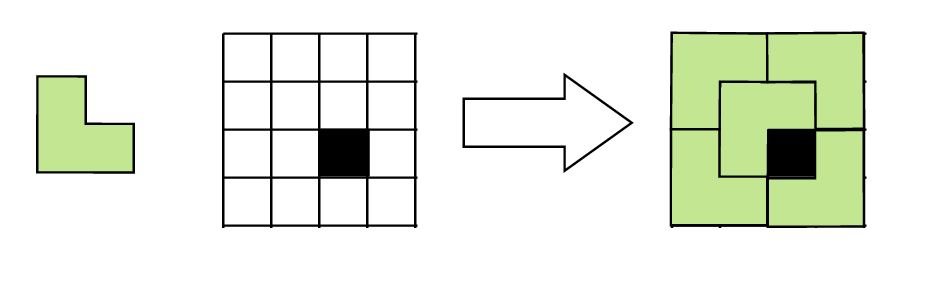
\includegraphics[scale=0.7]{diagrams/tiling.png}
    \caption{You are given $L$-shaped domino pieces (in light green) and a grid, and you are asked to find a way to tile the entire grid (excluding the black square). An example of a valid tiling is shown on the right.}
    \label{fig:my_label}
\end{figure}
\noindent 
\begin{enumerate}
    \item[(a)] Verify that, if $N = 2^k$, then $N^2 \equiv 1 \operatorname{ mod } 3$, and explain why this condition is necessary (while a priori not sufficient) for a valid tiling to exist.
    \item[(b)] Describe a procedure that allows you to find a valid tiling, given any input grid as above. You may give pseudocode but you are not required to.
    \item[(c)] Sketch a proof that your procedure works correctly.
\end{enumerate}
Note: every domino piece has the shape described above and covers exactly three squares, every input grid has exactly one excluded (black) square, but the location of the black square may change between input grids.
\end{problem}

\begin{solution}
    \noindent
    \begin{enumerate}[(a)]
        \item $N^2 = (2^k)^2 = 2^{2k}$ As we have $2^2 \equiv 1 \operatorname{mod} 3$, we can write $2^{2k}$ as $(2^2)^k \equiv 1^k \equiv 1 \operatorname{mod} 3$. This condition is necessary as each domino piece covers 3 squares, and the grid has $N^2$ squares.
        To cover the entire grid except for one square, the total number of squares must be one more than a multiple of 3, which must be ensured by $N^2 \equiv 1 \operatorname{mod} 3$.
        \item We can use a recursive algorithm to find a valid tiling. The algorithm can be described as follows:
        \begin{enumerate}[(1)]
            \item Divide the grid into four subgrids of size $\frac{N}{2} \times \frac{N}{2}$ and place the domino piece at the center such that it does not cover the square that has a missing square. This makes all four subgrids have a missing square.
            \item Recursively apply the algorithm to each of the four subgrids until all squares are filled out.
        \end{enumerate}
        \item We can prove the correctness by induction: Assume the tiling procedure works correctly for a grid of size $2^k \times 2^k$ with one square excluded. We will prove it works for a grid of $2^{k+1} \times 2^{k+1}$.\\
         \textbf{Base case:} For $k = 1$, the grid is $2 \times 2$, and the tiling works.\\
         \textbf{Inductive step:} We can divide the grid into four subgrids of size $2^{k} \times 2^{k}$, and place the domino piece at the center such that it does not cover the square that has a missing square. This makes all four subgrids have a missing square. By applying the algorithm recursively to each of the four subgrids, we can fill out all squares. 
            By tiling each subgrid and having the central domino in place, we achieve successful tiling for each $2^k$ grid, and therefore the tiling works for $2^{k+1} \times 2^{k+1}$ grid.
    \end{enumerate}
\end{solution}

\newpage
\extraspace

\newpage
\begin{problem}[Benchmarking Insertion Sort]

After reading the correctness proof of insertion sort during discussion for week 1, Konstantinos is wondering how many times line 6 is performed for a given array. He could simply count, but it took too long for big arrays, so instead he wants you to write a faster algorithm to compute that result.

\begin{algorithm}
    \caption{Insertion Sort} 
    \begin{algorithmic}[1]
    \Statex \textbf{Input:} Array $A$
    \Statex \textbf{Output:} Array $A$ 
    
    \For{$j=2$ to $A$.length} 
        \State $key$ $=$ $A[j]$
        \State // Insert $A[j]$ into the sorted sequence $A[1..j-1]$.
        \State $i = j-1$
        \While{$i > 0$ and $A[i] > key$}
            \State $A[i+1] = A[i]$
            \State $i = i - 1$
        \EndWhile
        \State $A[i+1]$ $=$ $key$
    \EndFor
    \State \textbf{Return} $A$
    \end{algorithmic}
\end{algorithm}
\noindent{\bf Input:} The first line contains a single integer $N$, the size of the array. In the next line there are $N$ numbers, from $1$ to $N$.\\
\\
{\bf Output:} A single number, how many times line 6 of insertion sort would be executed on this array. \\
\\
{\bf Submission:} In \href{https://www.gradescope.com/courses/753885/}{Gradescope} upload a single Python file. Skeleton code to get you started can be found on Canvas. \\
\\
{\bf Testing:} Test case inputs and outputs are provided \href{https://uchicago.box.com/s/ebv1r1sjdrc0hn6nawzbuo6wv5ywq44o}{here}. To compare your output to the given output you can use the following command on Linux and MacOS Terminal
\begin{verbatim}
pypy3 benchmarking_insertion.py <testcases/input01.txt | diff testcases/output01.txt -
\end{verbatim}
{\bf Limits:}\\
$N \leq 1.000.000$\\
$T \leq 2s$
\end{problem}
\begin{minipage}[t]{.20\textwidth}
Sample Input
\begin{verbatim}
5
2 5 3 4 1
\end{verbatim}
\end{minipage}% This must go next to `\end{minipage}`
\begin{minipage}[t]{.20\textwidth}
Sample Output
\begin{verbatim}
6
\end{verbatim}
\end{minipage}

\vspace{5mm}
\end{document}